\documentclass[11pt]{article}

\oddsidemargin=0.25truein \evensidemargin=0.25truein
\topmargin=-0.5truein \textwidth=6.0truein \textheight=8.75truein

\usepackage{graphicx}
\usepackage{verbatim}
\usepackage{booktabs}
\usepackage{comment}
\usepackage[dvipdfm]{hyperref}
\urlstyle{rm}   % change fonts for url's (from Chad Jones)
\hypersetup{
    colorlinks=true,        % kills boxes
    allcolors=blue,
    pdfsubject={ECON-UB233, Macroeconomic foundations for asset pricing},
    pdfauthor={Dave Backus @ NYU},
    pdfstartview={FitH},
    pdfpagemode={UseNone},
%    pdfnewwindow=true,      % links in new window
%    linkcolor=blue,         % color of internal links
%    citecolor=blue,         % color of links to bibliography
%    filecolor=blue,         % color of file links
%    urlcolor=blue           % color of external links
% see:  http://www.tug.org/applications/hyperref/manual.html
}

\renewcommand{\thefootnote}{\fnsymbol{footnote}}

% document starts here
\begin{document}
\parskip=\bigskipamount
\parindent=0.0in
\thispagestyle{empty}
{\large ECON-UB 233 \hfill Dave Backus @ NYU}

\bigskip\bigskip
\centerline{\Large \bf Properties of the Pricing Kernel}
\centerline{(Started: December 10, 2011; Revised: \today)}

\bigskip
We retrace the steps of the last thirty years of macro-finance research on asset returns.
The term macro-finance means
(a)~we're interested in returns on aggregate assets like bonds and equity indexes
and (b)~we'd like to account for those returns with a macroeconomic model,
such as one with a representative agent.

A quick summary would go like this:
%
\begin{itemize}
\item Mehra and Prescott's equity premium paper (JME, 1985).
They showed that a representative agent model with power utility
can't account for the observed average excess return on equity
with reasonable risk aversion.
\item Hansen and Jagannathan (JPE, 1991) narrowed the problem to the pricing kernel.
The so-called HJ bound shows that the dispersion of the pricing kernel
is bounded below by the Sharpe ratio of any traded asset, including equity.
Therefore the issue with the equity premium has to do with the pricing kernel,
not the dividends to which equity is a claim.
I like a variant of this result, in which dispersion is measured
by entropy, something we'll define when we get to it.
\end{itemize}
%
In short, when we observe high excess returns or Sharpe ratios,
they tell us that there must be a lot of dispersion in the pricing kernel.
Any model lacking such dispersion is dead from the start.
With power utility, that typically means high risk aversion,
which brings us back to what degree of risk aversion is reasonable.
The evident problems with the representative agent power utility model
has led to all kinds of interesting work.

In all of this, we'll use a timing in which $t$ is now
and $t+1$ is later.
With time measured in years, $t+1$ would be one year from now.
That's similar to what we've done so far,
but with $t$ taking the place of date 0 and $t+1$ taking the place of date 1.


\subsection*{Evidence:  properties of excess returns and consumption growth}

Table 1 and figure 1 summarize 100+ years of US asset returns and consumption
growth,
annual data for the period 1889-2009.
Figure 1 makes it clear that the variation in excess returns on the S\&P 500 index
and its predecessors
are closely related to variation in aggregate consumption growth.
In that sense, this is a macroeconomic phenomenon.

Beyond this, we have some useful summary statistics.
We compute most of them in levels of returns ($r^1$ and $r^e$)
and logs ($\log r^1$ and $\log r^e$).
The same with consumption growth:  $g_{t+1} = c_{t+1}/c_t$
and $\log g_{t+1}$.
In levels, the mean short or riskfree rate is 2\% ($r^1 = 1.02$).
The mean excess return on equity is 5.7\% ($r^e - r^1 = 0.057$).
For later reference, the Sharpe ratio is the mean excess return divided
by its standard deviation.
For equity, that's $ 0.0571/0.1873 = 0.3049$.
(That's way to many digits, but I wanted to be clear about the calculation.)
These numbers, or something like them, are targets for numerical examples
of theoretical models.

Since many of our models are loglinear, we report similar numbers in logs.
In logs, the mean short rate is 1.8\% ($\log r^1 = 0.018$)
and the mean equity premium is about 4.0\% ($\log r^e - \log r^1 = 0.04$).
I've rounded off most of these numbers to keep things clean.

We'll use the properties of consumption growth shortly.

\subsection*{The nature of research}

*******

Question.  Then use data and theory to provide an answer.  


\subsection*{The riskfree rate and equity premium puzzles}

Next up:  we consider models in which we can generate theoretical asset returns
and compare them to what we see in US data.
We'll use our usual setup, a representative agent economy
with power utility, a given random distribution of consumption
growth, and dividends tied to consumption growth.
We can come back later and see if that's a problem.

Our first example is as simple as we can make it.
There are two dates, $t$ and $t+1$.
There are two states at $t+1$, call them $ z \in \mathcal{Z} = \{-1, 1\}$,
each with probability one-half, $p(-1) = p(1) = 1/2$.
(Why this?  We could use $\mathcal{Z} = \{1,2\}$ if we prefer, but this is cleaner
in the Matlab program.)
Let us say that log consumption growth is
\begin{eqnarray*}
    \log g_{t+1}(z) &=& \mu + \sigma z .
\end{eqnarray*}
With this setup, it's clear that the mean and standard deviation of log consumption growth
are $\mu$ and $\sigma$, respectively.
Looking at Table 1, we use the values $\mu = 0.02$ and $\sigma = 0.035$.

Asset pricing follows from a pricing kernel and the dividends or cash flows
of the relevant assets.
With a representative agent and power utility, the pricing kernel follows
from consumption growth:
\begin{eqnarray*}
    m_{t+1} (z) &=& \beta g_{t+1}(z)^{-\alpha} .
\end{eqnarray*}
The assets of interest are the riskfree bond, which has a dividend of 1 in all states,
and ``equity,'' which has a dividend of $g_{t+1}(z)$ in state $z$.
The riskfree rate is $r^1 = 1/q^1$ where
\begin{eqnarray*}
    q^1 &=& E (m_{t+1} )  \;\;=\;\; \sum_z p(z) m(z) .
\end{eqnarray*}
Equity is a claim to consumption growth, so its price is
\begin{eqnarray*}
    q^e &=& E (m_{t+1} g_{t+1} )  \;\;=\;\; \sum_z p(z) m(z) g(z) .
\end{eqnarray*}
Its return is $ g(z)/q^e$, so its mean return is $E(r^e) = E (g)/q^e$.
The equity premium is $ E(r^e) - r^1$.
In this environment, each of these calculations is easily done in Matlab.

So what do we get?
We set $\beta = 0.99$ to get started.
If $\alpha = 2$, the riskfree rate $r^1$ is 1.0383, which well above our target of 1.020,
and the equity premium 0.0025, which is well below our target of 0.057.
We could fix the riskfree rate by raising $\beta$,
but this has its limits (1?).
If we raise $\alpha = 5$, the riskfree rate is 1.0995,
which is even higher,
and the equity premium rises only to 0.0067.
If we take this range of $\alpha$ to be reasonable, we're stuck.

[See Matlab program for computations.]


Our second example is based on our lognormal environment,
which we'll try to match to properties of log returns.
The advantage over the two-state setup is that we can see all the calculations,
but its properties are similar.
Let us say then that $\log g_{t+1} \sim \mathcal{N}(\kappa_1, \kappa_2)$.
(Sorry for the change in notation, it's habit.)
That gives us
$\log m_{t+1} \sim \mathcal{N}(\log \beta - \alpha \kappa_1, \alpha^2 \kappa_2)$.


We'll use a convenient shortcut, which I got from Andy Abel.
Consider a claim to $g_{t+1}^\lambda$.
If $\lambda = 0$, we get the riskfree bond,
and if $\lambda = 1$ we get equity.
The price of this asset is
\begin{eqnarray*}
    q(\lambda) &=& \beta E \left( g_{t+1}^{\lambda-\alpha} \right)
            \;\;=\;\; \beta \exp \left[ (\lambda - \alpha) \kappa_1
                    + (\lambda-\alpha)^2 \kappa_2 /2 \right] .
\end{eqnarray*}
That gives us
\begin{eqnarray*}
   \log r^1  &=& - \log \beta + \alpha \kappa_1 - \alpha^2 \kappa_2/2 \\
   E (\log r^e ) &=& - \log \beta + \alpha \kappa_1 - (\alpha-\lambda)^2 \kappa_2/2 \\
   E (\log r^e - \log r^1 )
        &=& [ \alpha^2 -  (\alpha-\lambda)^2 ] \kappa_2/2  \\
        &=& (2\alpha - 1)  \kappa_2/2 \;\; \mbox{ when } \;\; \lambda = 1 .
\end{eqnarray*}
You can see both puzzles right here.
The riskfree rate is quadratic in $\alpha$.
At moderate values, it increase with $\alpha$, so the riskfree rate will be too high.
(You can add numbers to make this more precise.)
But if $\alpha$ gets big enough, the impact of the variance term will bring it down again.
The equity premium, on the other hand, is increasing in $\alpha$.
If we make $\alpha$ large enough, we can account for any equity premium we like.
Using $\kappa_1 = 0.035^2 $,
We'll hit the equity premium of 0.0400 (in logs, remember) at
\begin{eqnarray*}
    2 \alpha - 1 &=& 2 (0.0400) / (0.035^2) ,
\end{eqnarray*}
or $\alpha = 33.15$.

Both examples make the same point:
that we can't account for the observed equity premium unless
we use a large value of $\alpha$.
If $\alpha = 33$ reasonable?
There's some debate about that,
but our own thought experiment in class suggests it's a bit high.
People with that kind of risk aversion won't be willing to take much risk.

Where do we go from here?
When we discussed this in class,
you made a number of good suggestions.
Among them:
(i)~consider a more complex distribution of dividends;
(ii)~ditto consumption growth;
(iii)~use some kind of ``friction'' so that the risks faced by an individual
are greater than those evident in aggregate consumption; and
(iv)~allow different preferences.
All of these are good ideas.
The first one we'll rule out shortly.
The others take more advanced tools than we have at present,
but we may come back to them if we have time.


\subsection*{The Hansen-Jagannathan bound}

If we think of the equity premium as a problem, the question is where its roots lie.
The answer, in good part, is the pricing kernel.
In this section and the next we derive two bounds on the variability of the pricing kernel.
Observed risk premiums give us lower bounds on the variability of the pricing kernel,
whatever it might be.
With power utility, the point is that you need lots of risk aversion to get enough
variability.

The first bound comes from Hansen and Jagannathan.
They note that the return on any asset $j$ satisfies
\begin{eqnarray}
    E \left( m r^j \right) &=& 1 .
    \label{eq:foc}
\end{eqnarray}
If we take two assets, say $j$ and $1$,
then the excess return $x = r^j - r^1$ satisfies
\begin{eqnarray*}
    E \left( m x \right) &=& 0 .
\end{eqnarray*}
That's true for any two returns.

Now let's see where this leads.
Expanding terms and applying the definition of the covariance gives us
\begin{eqnarray*}
    E \left( m x \right) &=& E (m) E(x) + \mbox{\it Cov\/}(m,x)
            \;\;=\;\; E (m) E(x) + \rho_{mx} \mbox{\it Std\/}(m) \mbox{\it Std\/}(x) .
\end{eqnarray*}
Here $\rho_{mx}$ is the correlation between $m$ and $x$
and $\mbox{\it Std\/}$ is the standard deviation.
Since the absolute value of the correlation is less than one,
we have
\begin{eqnarray*}
  \frac{| E(x)|}{ \mbox{\it Std\/}(x)} &\leq& \frac{ \mbox{\it Std\/}(m)}{E(m)} .
\end{eqnarray*}
This is the HJ bound.
It says that the Sharpe ratio (the left side) places an lower bound
on the dispersion of the pricing kernel.
Dispersion here is the ratio of the pricing kernel's standard deviation to its mean.
The mean is close to one (the price of a one-period bond),
so it's more or less the standard deviation.


\subsection*{The entropy bound}

The entropy bound has a similar flavor.
Here we define the pricing kernel's entropy $H(m)$ by
\begin{eqnarray*}
    H(m) &=& \log E(m) - E \log m .
\end{eqnarray*}
Since $\log$ is a concave function,
Jensen's inequality assures us that $H(m) \geq 0$,
with equality only if $m$ is constant.
It is, therefore, a measure of dispersion or variability.

You can see how it works in the lognormal case.
If $ \log m \sim \mathcal{N}(\kappa_1,\kappa_2)$,
then
\begin{eqnarray*}
    H(m) &=& (\kappa_1 + \kappa_2/2) - \kappa_1
            \;\;=\;\; \kappa_2/2 ,
\end{eqnarray*}
the variance over two.

The bound connects the entropy of the pricing kernel to expected excess returns in logs.
We start again with the pricing relation (\ref{eq:foc}).
If we take the log of $mr$, then Jensen's inequality tells us that
\begin{eqnarray*}
    E \left[ \log ( m r^j )\right] &=& \log (1) \;\;=\;\; 0 ,
\end{eqnarray*}
or
\begin{eqnarray*}
    E  \log r^j  &\leq& - E \log m \;\;=\;\; E \log m^{-1} .
\end{eqnarray*}
The highest possible return, in other words, is $r = 1/m$.

That gives us the second term in entropy, but what about the first?
We have
\begin{eqnarray*}
     \log E (m)  &=& \log q^1 \;\;=\;\; - \log r^1 .
\end{eqnarray*}
Together we have
\begin{eqnarray*}
    E  \log r^j - \log r^1  &\leq& \log E(m) - E \log m  \;\;=\;\; H(m) .
\end{eqnarray*}
In words: excess returns place a lower bound on the entropy
of the pricing kernel.

If $\log m $ is normal, then this places a lower bound on its variance $\kappa_2$:
\begin{eqnarray*}
    H(m) &=& \kappa_2/2 \;\;\geq\;\; 0.0400 .
\end{eqnarray*}
More generally, entropy will incorporate all the high-order cumulants of $\log m$.
Recall that $\log m$ has the cumulant generating function
\begin{eqnarray*}
    k(s; \log m) &=& \log E \left( e^{s \log m} \right) .
\end{eqnarray*}
The first term in the definition of entropy is therefore $k(1; \log m)$.
If the cgf has the power series expansion
\begin{eqnarray*}
    k(s; \log m) &=& \kappa_1 s + \kappa_2 s^2/2 + \kappa_3 s^3 / 3! + \kappa_4 s^4/ 4! + \cdots
\end{eqnarray*}
for some suitable range of $s$,
then
\begin{eqnarray*}
    H(m)  &=& \kappa_2 /2 + \kappa_3 / 3! + \kappa_4 / 4! + \cdots .
\end{eqnarray*}
The first term is the lognormal term.
The others illustrate the potential benefit of departing from normality,
since they can increase entropy even when we hold the variance constant.
Our colleague Stan Zin refers to this as the {\it never-a-dull-moment conjecture\/}:
if a model doesn't work, you can in principle fix it up by adding enough
high-order cumulants.
Whether that's reasonable is another matter, but it's an interesting
illustration of the benefits of going beyond the normal distribution.
Note in particular that positive skewness ($\kappa_3 > 0$) and kurtosis $\kappa_4 > 0$)
increase entropy.


The $\kappa_j$'s here are cumulants of $\log m$,
but with power utility, it's not hard to show that they're connected to cumulants
of $\log g$:
\begin{eqnarray*}
    \kappa_j (\log m) &=& (-\alpha)^j  \kappa_j (\log g), \;\;  j\geq 2.
\end{eqnarray*}
You can see here that for odd cumulants to make a positive contribution to entropy,
the cumulants of log consumption growth must be negative.
Thus negative skewness in $\log g$ leads to positive skewness in $\log m$.
Amir Yaron notes that the power of $\alpha$ allows small cumulants in log consumption growth
to become large cumulants in the log pricing kernel.
We refer to that as {\it Yaron's bazooka\/} in his honor.

Before finishing, here's a calculation related to the equity premium.
In the normal case,
$\kappa_2(\log m) = \alpha^2 \kappa_2(\log g)$.
The bound based on the equity premium therefore implies
\begin{eqnarray*}
    H(m) &=& \alpha^2 \kappa_2(\log g)/2 \;\;\geq\;\; 0.0400 .
\end{eqnarray*}
With $\kappa_2 = 0.035^2 $ (Table 1),
that implies $\alpha \geq 8.08$.
This is lower than our equity premium calculation,
but then it's a lower bound.


\subsection*{Bottom line}

The equity premium, the Hansen-Jagannathan bound, and the entropy bound
all point to variability in the pricing kernel as a key issue for asset pricing models
--- all of them.
Representative agent models with power utility have difficulty with all three,
because aggregate consumption growth has a modest amount of variability
and large values of the risk aversion parameter are thought by many to be
implausible.
The representative agent paradigm retains one important strength:
the connection between returns and business cycles
is a feature of both these models and the data (Figure 1, for example).
The challenge for the future is to retain this strength
yet deliver larger risk premiums.


% ----------------------------------------------------------------------
\pagebreak
{\large\bf Table 1 \\ Properties of US real asset returns and consumption growth}

\bigskip
\tabcolsep=10pt
\begin{tabular}{lrrrr}
\toprule
Asset       & Mean  & Std Dev  & Skewness & Ex Kurt \\
\midrule
\multicolumn{3}{l}{\it Properties of levels} \\
Consumption growth $g$ \phantom{xxxxxxxxxxx}
                        & 1.0207  &  0.0356  & --0.1886 & 0.9434 \\
Short rate $r^1 $       & 1.0198  &  0.0580  &  0.4174  &  2.8122 \\
Equity return $r^e$     & 1.0769  &  0.1846  & --0.0898 & --0.1035 \\
Excess return $r^e-r^1$ & 0.0571  &  0.1873  & --0.2095 &   0.2809 \\
\midrule
\multicolumn{3}{l}{\it Properties of logs} \\
Consumption growth $\log g$  & 0.0198 & 0.0350 & --0.3433 & 1.1112  \\
Short rate $\log r^1 $       &  0.0180  & 0.0566  &  0.0380   & 2.3976 \\
Equity return $\log r^e$     &  0.0587  & 0.1795  & --0.6134  &  0.4311 \\
Excess return $\log r^e - \log r^1$ &  0.0407 & 0.1812 & --0.7157 & 0.9065 \\
\bottomrule
\end{tabular}

Source:  Shiller, website, updated.
Data covers the period 1889-2009, annual.
Returns are real:  nominal returns minus inflation.
Equity is the S\&P 500 and its predecessors.
Consumption is per capita.

\pagebreak
{\large\bf Figure 1 \\ US real asset returns v. consumption growth, 1889-2009}

\bigskip
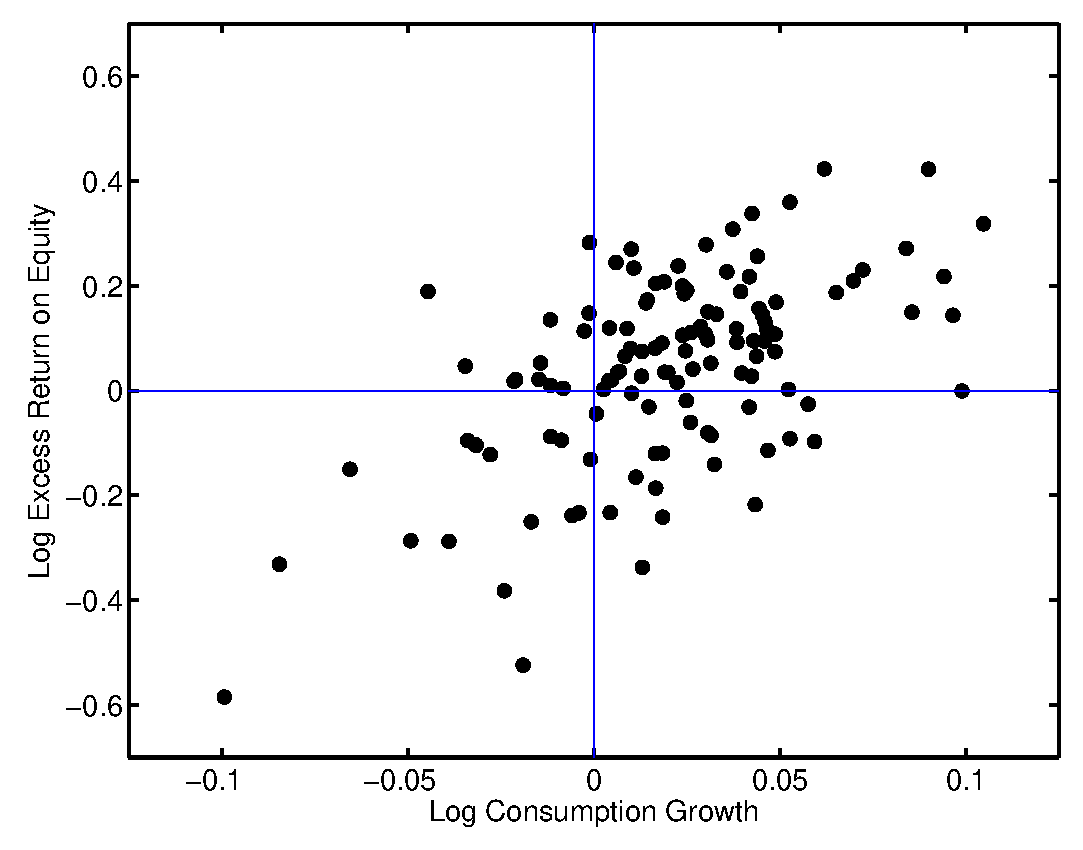
\includegraphics[width=\textwidth]{scatter_gxr.eps} \\


\vfill \centerline{\it \copyright \ \number\year \
NYU Stern School of Business}
\end{document}
